
\chapter{Funció de multiresolució aplicada a les sèries temporals}


En aquest capítol definim la multiresolució com una funció que
s'aplica a una sèrie temporal i retorna una nova sèrie temporal.
Aquesta nova sèrie temporal és el resultat d'aplicar, en l'àmbit dels
\glspl{SGST}, un esquema de multiresolució a la sèrie temporal
original. Aquesta aplicació té el mateix efecte que utilitzar, en
l'àmbit dels \glspl{SGSTM}, una sèrie temporal multiresolució amb
aquest esquema. Però les aplicacions que resulten d'ambdós casos no
tenen les mateixes propietats.

En el model de \gls{SGSTM} s'ha definit la
multiresolució com una estructura de base de dades en què cal
emmagatzemar i tractar una sèrie temporal. En canvi, ara observem la
multiresolució com una funció simple que opera sobre una sèrie
temporal i no té capacitats d'emmagatzematge d'informació.  D'aquesta
manera, una funció de multiresolució permet:
\begin{itemize}

\item Plantejar problemes on la multiresolució sigui gestionada com
  una consulta sobre una sèrie temporal, és a dir com una operació
  dels \gls{SGST} que calcula parelles d'agregació d'atributs i
  resolucions temporals per a una sèrie temporal.

\item Dissenyar sistemes duals de \glspl{SGSTM} i \glspl{SGST} amb
  operacions de consulta multiresolució, en els quals una sèrie
  temporal és emmagatzemada doblement en tots dos sistemes.

\item Estudiar altres implementacions de la consulta de multiresolució, p.ex. para\l.lelisme. (vegeu secció implementació \todo{})



\end{itemize}





\section{Funció de multiresolució}
\label{sec:multiresolucio:funcio}


%es podria implementar com una operació de summarize?



En el model de \gls{SGSTM} hem definit un model de dades per a
gestionar sèries temporals multiresolució. Aquest model té una
estructura que emmagatzema la informació d'una sèrie temporal en una
forma determinada: la de multiresolució.  La definició com a
\gls{SGSTM} té com a objectius l'emmagatzematge compacte de les dades
i la selecció de la informació ja preparada per a consultes
posteriors.

Així, aquest model té capacitats de computació
sincronitzada o en línia (\emph{online}) amb el temps i té
característiques dels sistemes que tracten fluxos de dades (\emph{data
  stream}); és a dir dades que s'estan adquirint contínuament i cal
anar computant al mateix temps que es van adquirint. Això no treu,
però, que de manera més simplificada també es pugui treballar amb un
\gls{SGSTM} en temps diferit (\emph{offline}), és a dir que
s'emmagatzemin les dades adquirides i en el moment que es vulgui
aplicar-hi la consolidació.




Això no obstant, podem simplificar el problema de càlcul de
multiresolució en temps diferit com una consulta en un \gls{SGST} de
transformació d'una sèrie temporal a una nova sèrie temporal.

\todo{ref a la definició d'esquema multiresolució def:sgstm:esquema}

És a dir, sigui $S=\{m_0,m_1,\dotsc,m_k\}$ una sèrie temporal, $M$ una
sèrie temporal multiresolució i $e = \{ (\delta_0,f_0,\tau_0,k_0),
\ldots, (\delta_d,f_d,\tau_d,k_d)\}$ els paràmetres de l'esquema de
multiresolució de $M$. Afegim totes les mesures de la sèrie temporal a
la multiresolució, $\forall m \in S:$
\[
M_0=\glssymbol{addM}(M,m_0),M_1=\glssymbol{addM}(M_0,m_1),\dotsc,M_k=\glssymbol{addM}(M_{k-1},m_k)
\]
i la consolidem fins que no sigui consolidable, sigui
$c\in\glssymbol{not:N}:$
\[
M'_0=\glssymbol{consolidaM}(M_k),\dotsc,M'_{c}=\glssymbol{consolidaM}(M'_{c-1}),M'=\glssymbol{consolidaM}(M'_{c})
\]
on $M_k,M'_{0},\dotsc,M'_{c-1},M'_{c}$ són consolidables i $M'$ no és
consolidable.  Consultem la sèrie temporal multiresolució amb les dues
consultes bàsiques, les quals retornen sèries temporals,
$S'=\glssymbol{not:sgstm:serietotal}(M')$ i $S_{\delta
  f}'\glssymbol{not:sgstm:seriedisc}=(M',\delta,f)$ on $\delta$ i $f$
són dos paràmetres de l'esquema de multiresolució de $M$ que van
associats amb els altres dos corresponents $\tau$ i $k$.



Plantegem les funcions de transformació de la sèrie temporal original
a les consultades. És a dir, les funcions que anomenem
$\glssymbol{not:sgstm:dmap}$ i $\glssymbol{not:sgstm:multiresolucio}$
i que ens permeten calcular:

\[
\glssymbol{not:sgstm:dmap}: S \times \delta \times f \times \tau \times k \longrightarrow
S'_{\delta f}
\]


\[
 \glssymbol{not:sgstm:multiresolucio}: S \times e  \longrightarrow S'
\]



Definim la consulta de selecció de disc dels \gls{SGSTM} a partir del
mapatge dels \gls{SGST} de manera que, en computació per temps
diferit, són equivalents
\[
\glssymbol{not:sgstm:seriedisc}(M',\delta,f) \equiv
\glssymboldef{not:sgstm:dmap}(S,\delta,f,\tau,k)
\]


\begin{definition}[mapa de \glssymbol{not:sgstm:seriedisc}]
  Sigui $S$ una sèrie temporal, $M$ una sèrie temporal multiresolució
  amb esquema $e$ i $(\delta,f,\tau,k)\in e$ els paràmetres de
  multiresolució d'una subsèrie resolució. L'expressió de
  $\glssymbol{not:sgstm:seriedisc}(M',\delta,f)$ com a mapa d'una sèrie
  temporal és $\glssymboldef{not:sgstm:dmap}(S,\delta,f,\tau,k)=
  \glssymbol{not:sgst:map}(S_I,\glssymbol{not:sgst:fmap})$ on
  \[
  \glssymbol{not:sgst:fmap}: m_i\mapsto f(S, [T(m_i)-\delta,T(m_i)]),
  \]
  \[
  S_I = \{ (t,\infty) | t\in T_I  \},\;  t_M = T(\max(S)),
  \]
  \[
  T_I = \{ t_I = \tau+n\delta | n\in\glssymbol{not:Z}, t_M - k\delta <
  t_I \leq t_M \}.
  \]
\end{definition}








Definim la consulta de sèrie temporal total dels \gls{SGSTM} a partir
del plegament dels \gls{SGST} de manera que, en computació per temps
diferit, són equivalents
\[
\glssymbol{not:sgstm:serietotal}(M') \equiv \glssymbol{not:sgstm:multiresolucio}(S,e)
\]

\begin{definition}[plec de \glssymbol{not:sgstm:serietotal}]
  Sigui $S$ una sèrie temporal i $M$ una sèrie temporal multiresolució
  amb esquema $e = \{ (\delta_0,f_0,\tau_0,k_0), \ldots,
  (\delta_d,f_d,\tau_d,k_d)\}$, el qual es pot observar com una sèrie
  temporal multivaluada.  L'expressió de
  $\glssymbol{not:sgstm:serietotal}(M)$ com a plec d'una sèrie
  temporal és $\glssymboldef{not:sgstm:multiresolucio}(S,e)=
  \glssymbol{not:sgst:ofold}(e,\{\},\glssymbol{not:sgst:ffold},\min)$
  on $\glssymbol{not:sgst:ffold}: S_i \times (\delta_c,f_c,\tau_c,k_c)
  \mapsto S_i ||
  \glssymbol{not:sgstm:dmap}(S,\delta_c,f_c,\tau_c,k_c)$.

  Així, el plec de \glssymbol{not:sgstm:serietotal} és la concatenació de
  tots els \glssymbol{not:sgstm:dmap} possibles per l'esquema $e$
  ordenats per $\delta$, assumint que $e$ no conté $\delta$ repetits.
\end{definition}



En resum: en temps diferit, s'insereixen les mateixes mesures a un
\gls{SGST} i a un \gls{SGSTM}. Per una banda es consolida el
\gls{SGSTM} i s'obté la sèrie total i per altra banda es consulta la
multiresolució en el \gls{SGST}. Aleshores s'obté la mateixa sèrie
temporal. 


Vegem en dos exemples el càlcul de la funció de multiresolució. \todo{millor que hi hagi també el càlcul amb \gls{SGSTM} i així es vegi l'equivalència?}

\begin{example}
  \label{ex:multiresolucio:dmap}
  Sigui la sèrie temporal $S=\{(1,0),(3,1),(6,0),(10,1)\}$ i els
  paràmetres de multiresolució
  $(\delta_0=5,f_0=\glssymbol{not:sgstm:maxdd},\tau_0=0,k_0=2)$.  El
  mapa de \glssymbol{not:sgstm:seriedisc} és una sèrie temporal $S'=
  \glssymboldef{not:sgstm:dmap}(S,5,0,\glssymbol{not:sgstm:maxdd},2)$
  on $S'=\{(5,1),(10,1)\}$. Expressem el càlcul pas a pas, a la
  \autoref{fig:multiresolucio:dmap} es visualitzen en taula les sèries
  temporals corresponents:
  \begin{enumerate}
  \item El primer pas és obtenir els instants de temps que
    s'emmagatzemarien al disc d'una sèrie temporal
    multiresolució. Així, els instants de consolidació possibles són
    $T_I'=\{\tau+n\delta|n\in\glssymbol{not:Z}\}=
    \{\ldots,-5,0,5,10,15,\ldots\}$. Però un cop consolidat el disc
    només hi haurà els $k=2$ més recents abans de $t_M=T(\max(S))=10$,
    és a dir $T_I=\{t_I'\in T_I'|t_M - k\delta < t_I \leq
    t_M\}=\{5,10\}$.

  \item El segon pas és obtenir a partir de $T_I$ la sèrie temporal
    $S_I$ que es correspon amb la sèrie temporal que s'inicialitzaria
    al disc encara amb valors desconeguts,
    $S_I=\{(5,\infty),(10,\infty)\}$.



  \item El tercer pas és calcular la funció d'agregació a $S$ per a
    cada intervals de consolidació del disc de la forma
    $[T(m_i)-\delta,T(m_i)]$ on $m_i\in S_i$, és a dir $f(S,[0,5])$ i
    $f(S,[5,10])$. A tal efecte utilitzem el mapa sobre $S_I$ per a
    calcular la sèrie temporal resultant $S'=\{ (5,f(S,[0,5])),
    (10,f(S,[5,10])) \}$.

    Podríem calcular un pas entremig que es correspon amb les sèries
    temporals que hi hauria en el buffer abans de cada instant de
    consolidació. Així, per a cada $T(m_i)$ hi hauria la sèrie
    temporal $S[T(m_i)-\delta,T(m_i)]$, és a dir $S_B=\{
    (5,S[0,5],(10,S[5,10]) \}$.
  \end{enumerate}



\begin{figure}[tp]
  \centering
  \begin{tabular}[c]{|c|c|}
    \multicolumn{2}{c}{$S$} \\ \hline
    $t$  & $v$ \\ \hline
    1  & 0 \\
    3  & 1 \\
    6  & 0 \\
    10  & 1 \\ \hline
  \end{tabular} \qquad
  \begin{tabular}[c]{|c|c|}
    \multicolumn{2}{c}{$S_I$} \\ \hline
    $t$  & $v$ \\ \hline
    5  & $\infty$ \\
    10  & $\infty$ \\ \hline
  \end{tabular} \qquad
  \begin{tabular}[c]{|c|c|}
    \multicolumn{2}{c}{$S_B$} \\ \hline 
    $t$  & $v$ \\ \hline
    5  &  \raisebox{0pt}[1ex+\height][1ex+\depth]{\begin{tabular}[c]{|c|c|}\hline $t$  & $v$ \\ \hline 1&0\\ 3&0 \\\hline  \end{tabular}} \\\hline
    10  & \raisebox{0pt}[1ex+\height][1ex+\depth]{\begin{tabular}[c]{|c|c|}\hline $t$  & $v$ \\ \hline 6&0\\ 10&1 \\\hline  \end{tabular}} \\ \hline
  \end{tabular} \qquad
 \begin{tabular}[c]{|c|c|}
    \multicolumn{2}{c}{$S'$} \\ \hline
    $t$  & $v$ \\ \hline
    5  & 1 \\
    10  & 1\\ \hline
  \end{tabular}
  \caption{Taules de les sèries temporals per l'operació de mapa de  \glssymbol{not:sgstm:seriedisc}}
  \label{fig:multiresolucio:dmap}
\end{figure}
 
\end{example}

\begin{example}
  Sigui la sèrie temporal $S=\{(1,0),(3,1),(6,0),(10,1)\}$ i l'esquema
  de multiresolució
  $e=\{(\delta_0=5,f_0=\glssymbol{not:sgstm:maxdd},\tau_0=0,k_0=2),
  (\delta_1=2,f_1=\glssymbol{not:sgstm:maxdd},\tau_1=0,k_1=3)\}$.
  El plec de $\glssymbol{not:sgstm:serietotal}$ és una sèrie temporal
  $S'= \glssymboldef{not:sgstm:multiresolucio}(S,e)$ on
  $S'=\{(5,1),(6,0),(8,0),(10,1)\}$. Expressem el càlcul pas a pas, a la
  \autoref{fig:multiresolucio:multiresolucio} es visualitzen en taula les sèries
  temporals corresponents:

  \begin{enumerate}
  \item En primer lloc es calcula la sèrie temporal pels paràmetres de
    multiresolució $\delta_0$:
    $S_{D0}=\glssymbol{not:sgstm:dmap}(5,\glssymbol{not:sgstm:maxdd},0,2)=\{(5,1),(10,1)\}$,
    com ja s'ha vist a l'\autoref{ex:multiresolucio:dmap}.

  \item En segon lloc, es calcula la sèrie temporal pels paràmetres de
    multiresolució $\delta_1$:
    $S_{D1}=\glssymbol{not:sgstm:dmap}(2,\glssymbol{not:sgstm:maxdd},0,3)=\{(6,0),(8,0),(10,1)\}$,
    de manera similar a $S_{D0}$.

  \item En tercer lloc es concatenen les sèries temporals per ordre de
    $\delta$: $\delta_1<\delta_0$. Així, $S'= S_{D1} || S_{D0}$.

  \end{enumerate}
  


\begin{figure}[tp]
  \centering
  \begin{tabular}[c]{|c|c|}
    \multicolumn{2}{c}{$S$} \\ \hline
    $t$  & $v$ \\ \hline
    1  & 0 \\
    3  & 1 \\
    6  & 0 \\
    10  & 1 \\ \hline
  \end{tabular} \qquad
  \begin{tabular}[c]{|c|c|}
    \multicolumn{2}{c}{$S_{D1}$} \\ \hline
    $t$  & $v$ \\ \hline
    5  & 1 \\
    10  & 1 \\ \hline
  \end{tabular} \qquad
  \begin{tabular}[c]{|c|c|}
    \multicolumn{2}{c}{$S_{D2}$} \\ \hline
    $t$  & $v$ \\ \hline
    6  & 0 \\
    8  & 0 \\
    10  & 1 \\ \hline
  \end{tabular} \qquad
  \begin{tabular}[c]{|c|c|}
    \multicolumn{2}{c}{$S'$} \\ \hline
    $t$  & $v$ \\ \hline
    5  & 1 \\
    6  & 0 \\
    8  & 0 \\
    10  & 1 \\ \hline
  \end{tabular}
  \caption{Taules de les sèries temporals per l'operació de plec de  \glssymbol{not:sgstm:serietotal}}
  \label{fig:multiresolucio:multiresolucio}
\end{figure}
 


\end{example}








\subsection{Demostració}

Cal demostrar l'equivalència formalment\todo{}





\chapter{Sistemes duals SGST+SGSTM}
\label{sec:multiresolucio:dual}


Una sèrie temporal es pot emmagatzemar i gestionar en un \gls{SGST} o
en un \gls{SGSTM}. També es pot plantejar un sistema dual de
multiresolució on una sèrie temporal es tracti alhora en un \gls{SGST}
i en un \gls{SGSTM}.

Les equivalències entre els \gls{SGSTM} i les funcions de
multiresolució aplicades a un \gls{SGST} permeten dissenyar sistemes
duals que tinguin propietats complementàries.  Així, aquests sistemes
duals ofereixen altres utilitats a la multiresolució més enllà de
l'orientació de compressió amb pèrdua mostrada a la secció??\todo{ref
  model sgstm}. A continuació:
\begin{itemize}
\item Dissenyem l'estructura d'aquests sistemes duals
\item Avaluem conceptes relacionats en l'àmbit genèric dels \gls{SGBD}
\item Mostrem les aplicacions que permeten
\end{itemize}




\subsection{Estructura}

Un sistema dual de multiresolució està format per un \gls{SGST} i un
\gls{SGSTM} on s'emmagatzemen les mateixes sèries temporals. A
cadascun s'hi pot fer les consultes pertinents de cada model per a les
sèries temporal. A més, s'obté el mateix resultat en els dos sistemes
per a les consultes que segueixin les restriccions de la funció de
multiresolució.


A la \autoref{fig:multiresolucio:dual} es mostra l'estructura d'un
sistema dual de multiresolució. L'usuari percep aquest sistema com un
\gls{SGST} on emmagatzema una sèrie temporal $S$ i hi gestiona les
consultes, on algunes d'aquestes consultes són de multiresolució o
treballen sobre sèries temporals $S'$ que provenen de la
multiresolució.  Internament hi ha un \gls{SGST} i un \gls{SGSTM} que
comparteixen l'entrada de mesures de la sèrie temporal. Així, quan
l'usuari so\l.licita la multiresolució $S'$, el sistema dual tant pot
calcular-la a partir del \gls{SGST} amb l'operació de
$\glssymbol{not:sgstm:multiresolucio}(S)$ com a partir del \gls{SGSTM}
amb l'operació de $\glssymbol{not:sgstm:serietotal}(M)$.  La mateixa
estructura també pot servir per al cas de les operacions de
$\glssymbol{not:sgstm:dmap}$ i les de
$\glssymbol{not:sgstm:seriedisc}$.


\begin{figure}
  \centering
  %\usetikzlibrary{shapes,arrows,positioning}
\begin{tikzpicture}[scale=0.8, every node/.style={transform shape}]

      \tikzset{
        mynode/.style={rectangle,rounded corners,draw=black, 
          very thick, inner sep=1em, minimum size=3em, text centered,
          groc},
        myarrow/.style={->, shorten >=1pt, thick},
        mylabel/.style={text width=7em, text centered},
        groc/.style={top color=white, bottom color=yellow!50},
        verd/.style={top color=white, bottom color=green!50},
        roig/.style={top color=white, bottom color=red!50},
      }  






 \node[mynode] (m) {$S$};

 \node[right=2cm of m] (mdins) {};

 \node[mynode, verd, above right=0.6cm and 1cm of mdins] (tsms) {\glstext{SGST}};

 \node[mynode, verd, below right=0.6cm and 1cm of mdins] (mtsms) {\glstext{SGSTM}};

 \node[rectangle,draw,minimum height=6cm,minimum width=9.5cm,right=-0.25cm of mdins] (dual) {};

\draw[shift=( dual.south west)]   
  node[above right] {sistema dual de multiresolució};






 \node[mynode,right=3cm of mtsms] (ts) {$S'$};



 \draw (m.east) -- (mdins.east) node[above right,at start]
 {afegeix$(m)$};

 \draw[myarrow] (mdins.east) -- (tsms.west);
 \draw[myarrow] (mdins.east) -- (mtsms.west);


 \draw[myarrow] (tsms) -- (ts) node[above,midway,sloped]
 {$\glssymbol{not:sgstm:multiresolucio}(S,\glssymbol{not:esquemaM})$}; 
 
 \draw[myarrow] (mtsms) -- (ts) node[above,midway,sloped]
 {$\glssymbol{not:sgstm:serietotal}(M)$};




 \node[right=6cm of tsms] (consdins) {};

 \draw (tsms) -- (consdins.center);
 \draw (ts) -- (consdins.center);

 \node[right=2.5cm of consdins] (consultes) {};
 \draw[myarrow] (consdins.center) -- (consultes) node[above,midway,sloped]
 {consultes};



\end{tikzpicture}



%%% Local Variables:
%%% TeX-master: "../main"
%%% End:

  \caption{Sistema dual de multiresolució: \gls{SGST}+\gls{SGSTM}}
  \label{fig:multiresolucio:dual}
\end{figure}


Cal comentar que el model de \gls{SGSTM} està dissenyat en base al
model de \gls{SGST} i per tant aquests primers sempre depenen dels
segons. No obstant això, cal no confondre aquesta dependència amb el
sistema dual, el qual gestiona una mateixa sèrie temporal independentment
en un \gls{SGSTM} i en un \gls{SGST}.




Tot i que per al sistema dual és equivalent calcular la sèrie temporal
resultant a partir del \gls{SGST} o del \gls{SGSTM}, no pot seguir el
mateix procediment en cada cas. Per una banda, la
$\glssymbol{not:sgstm:multiresolucio}(S)$ és una operació computada en
temps diferit; cada cop que s'afegeix una nova mesura cal tornar a
calcular tot el resultat. Per altra banda, la
$\glssymbol{not:sgstm:serietotal}(M)$ és una operació computada en
línia; és a dir seguint el flux d'adicions de les mesures.


El sistema dual dissenyat funciona a partir de l'adició de mesures, de
la mateixa manera que els \gls{SGSTM}. L'ordre d'arribada d'aquestes
mesures és crític en el sistema dual ja que un cop el \gls{SGSTM} s'ha
consolidat les dades més antigues que arribin no seran tingudes en
compte i per tant l'equivalència entre les consultes de \gls{SGST} i
\gls{SGSTM} ja no serà certa. Així doncs, si es vol mantenir
l'equivalència, el sistema dual dissenyat té aquestes dues
restriccions: només permet operacions d'adició i l'ordre d'adició és
important.  Més endavant a les aplicacions descriurem l'abast
d'aquestes restriccions.







\subsection{Conceptes relacionats}


\textcite{marz13:nosql13, marz14:bigdata} generalitzen un concepte
similar al de \gls{SGST} dual, ho emmarquen en l'àmbit dels \gls{SGBD}
per a \emph{Big Data}.  Proposen \gls{SGBD} dissenyats amb tres
nivells, que anomenen arquitectura \emph{Lambda}:
\begin{itemize}
\item Nivell \emph{batch}: Emmagatzema totes les dades originals i
  permet realitzar qualsevol consulta sobre aquestes dades. Preveu que
  algunes consultes operen sobre dades consultades prèviament, per
  tant en aquest nivell es gestionen també aquestes consultes
  precomputades, les quals a més es poden obtenir amb computació
  para\l.lela com per exemple amb Hadoop. Particularment, es considera
  que les dades originals són immutables, és a dir que les bases de
  dades només permeten afegir però no modificar.

\item Nivell \emph{server}: Emmagatzema les consultes precomputades i
  n'ofereix les dades per a altres consultes. Les consultes
  precomputades s'han de tornar a calcular periòdicament i en el
  nivell \emph{server} sempre hi ha la versió calculada més
  recent. Per tant, es preveu que les consultes precomputades no
  ofereixen la informació actualitzada al moment, sinó que hi ha un
  cert temps des que es modifiquen les dades originals fins que té
  impacte en les consultes.

\item Nivell \emph{speed}: Precomputa les mateixes consultes que el
  nivell \emph{batch} però incrementalment, és a dir cada cop que
  s'afegeix una dada nova les dades de la consulta \emph{speed}
  s'actualitzen adequadament.  Aquest nivell només s'usa per a dades
  recents per tal complementar el problema de les dades
  desactualitzades en els nivells \emph{batch} i \emph{server}.
\end{itemize}


Les consultes precomputades d'aquests sistemes semblen una bona
solució per a la computació de les vistes dels \gls{SGBDR}.  Una vista
és un àlies per a una expressió relacional, és a dir una consulta, que
s'utilitza en altres consultes. Per tant, una vista $v$ és una
operació $\text{op1}$ sobre unes $\text{dades}$,
$v:=\text{op1}(\text{dades})$, i s'utilitza una altra consulta
$\text{op2}(v)$ de manera que és equivalent a executar la consulta
$\text{op2}(\text{op1}(\text{dades}))$. Així doncs, el model de vistes
és similar a les consultes que es basen en altres consultes proposat
per \citeauthor{marz14:bigdata} o a les sèries temporals precomputades
que proposem.


En el model relacional \cite[cap.~10. Views]{date04:introduction8} es
considera, conceptualment, que les vistes no s'avaluen quan es
defineixen sinó cada cop que s'executa una consulta que hi opera.  En
les implementacions les vistes poden ser precomputades, aleshores
s'anomenen \emph{snapshots} o \emph{materialized views}, per tal
d'aconseguir un emmagatzematge temporal dels mateixos càlculs per a
diverses consultes. En el context de sistemes de suport a les
decisions, la precomputació també es preveu en el càlcul de taules
resum per a agregacions de les dades \cite[cap.~22. Decision
support]{date04:introduction8}.  Això no obstant, la precomputació de
vistes no sempre comporta una millor eficiència; el concepte de vista
del model permet la substitució algebraica i per tant permet
l'optimització global de la consulta i l'operació continguda a la
vista.



% PostgreSQL no té materialized views però aquí expliquen com definir-ne a partir de triggers. \url{http://tech.jonathangardner.net/wiki/PostgreSQL/Materialized_Views}.





Les vistes precomputades tenen associada una acció per actualitzar de
nou el seu valor, és a dir per a recalcular la consulta que contenen
quan les dades originals han canviat. En usar vistes precomputades cal
preveure el termini de validesa dels càlculs precomputats, com ocorre
en el nivell \emph{server} de l'arquitectura \emph{Lambda}. Així
doncs, les vistes precomputades es poden actualitzar de vàries
maneres:
\begin{itemize}

\item L'usuari decideix manualment quan s'han de tornar a computar. Per
  exemple, per a treballar durant un cert temps amb còpies immutables
  de les dades (\emph{snapshots}) sense haver de blocar la modificació
  de la base de dades \cite[\S{}10.5]{date04:introduction8}.

\item Es computen periòdicament, com també es proposa en el nivell
  \emph{batch} de l'arquitectura \emph{Lambda}.

\item Quan s'utilitzen per primer cop, es computen associades a un
  temps de termini a partir del qual si es tornen a utilitzar s'hauran
  de tornar a computar. 


\item Es computen cada cop que es modifiquen les dades amb les quals
  operen, és a dir quan les dades originals reben una operació
  d'afegir, de modificar o d'actualitzar es torna a computar tota la
  vista.

\item Quan es modifiquen les dades, s'aplica la mateixa operació a la
  vista precomputada; requereix especificar la instrucció
  d'actualització. És a dir, quan es modifiquen les dades originals
  amb una operació, $\text{mod}(\text{dades})$, es trasllada aquesta
  operació a la vista, $\text{mod}'(\text{dades})$, on cal determinar
  la relació entre $\text{mod}$ i $\text{mod}'$.  Aquesta translació
  és més senzilla quan només hi ha possibilitat d'operacions d'afegir
  noves dades però no de modificar-les: és el que es proposa en el
  nivell \emph{speed} de l'arquitectura \emph{Lambda} i el que admet
  el model de \gls{SGSTM} que proposem. \todo{s'ha d'estudiar la
    relació d'això amb els data stream}
% When data comes as an ordered sequence of instances it is called
% data stream, then specific \acro{DBMS} are designed to manage data
% stream data \cite{stonebraker05:sigmod}.  \acro{MTSMS} can take
% advantage of data stream orientation in order to simplify the
% consolidation process.  Assuming a time order acquisition of time
% series, the update of a \acro{MTSMS} only consists in the addition of
% new measures and the incremental consolidation of subseries. 
\end{itemize}



En resum, la sèrie temporal resultant dels sistemes duals pot ser
considerada com una vista calculada sobre les sèries temporals
originals. Aquesta vista pot ser precomputada, cosa que es pot fer de
diverses maneres: la funció de multiresolució l'ha de computar
totalment cada cop que s'afegeix una nova mesura i en canvi els
\gls{SGSTM} la computen incrementalment.  Aleshores aquestes vistes es
poden usar per a altres consultes que tinguin com a context
l'aproximació de multiresolució realitzada, o per a visualitzacions
gràfiques com les que ofereix RRDtool \cite{rrdtool}.






%Estudiar també Aurora
%http://www.cs.brown.edu/research/aurora/vldb03_journal.pdf
% Abadi, D., Carney, D., Cetintemel, U., Cherniack, M., Convey, C., Lee, S., Stonebraker, M., Tatbul, N., and Zdonik, S. Aurora: A New Model and Architecture for Data Stream Management. In VLDB Journal (12)2:120-139, August 2003.





\subsection{Aplicacions}


Les sèries temporals són dades que s'adquireixen contínuament i per
tant cada cop és més gran el volum de dades que s'ha d'emmagatzemar i
tractar. Aquest gran volum de dades és un problema per a operar amb
les sèries temporals i és un problema en els sistemes que tenen
l'emmagatzematge limitat. En aquest sentit, originalment hem
plantejat el model de \gls{SGSTM} per tal d'oferir una solució
d'emmagatzematge que comprimeix la informació seleccionant-ne una
multiresolució determinada.


Així, un \gls{SGSTM} implica un selecció d'informació i la informació
que no es considera importat és descartada. Aquests sistemes, per
tant, no són adequats quan totes les dades monitorades han de ser
emmagatzemades tal com s'adquireixen. Un cas d'aquests és quan no es
coneixen quines funcions d'agregació són les més escaients per a les
dades futures que s'adquiriran. Un altre cas és quan volem resoldre
consultes detallades sobre les dades, com per exemple: a quina hora
exacta ha ocorregut un esdeveniment.


Els sistemes duals de multiresolució ofereixen una solució per
emmagatzemar totes les dades però mantenint-ne una gestió de
multiresolució.  En el sistema dual, s'ha d'entendre el \gls{SGST} com
un emmagatzematge a llarg termini que no és consultat freqüentment;
així pot estar implementat com a \gls{SGBD} per a dades de gran volum
i basat en tècniques de compressió sense pèrdua, encara que tinguin
temps grans de descompressió. El \gls{SGSTM} s'ha d'entendre com un
emmagatzematge de compressió amb pèrdua que conté multiresolucions
precomputades de la sèries temporal.  El temps de còmput no és tant
crític en els \gls{SGSTM} perquè es reparteix al llarg del temps, és a
dir tal com es van adquirint les dades; més enllà del temps de còmput
de cada funció d'agregació d'atributs, el qual limita la quantitat de
multiresolucions diferents que pot gestionar un mateix \gls{SGSTM}.


En la compressió de dades multimèdia s'utilitza una tècnica de gestió
similar.  Les dades s'emmagatzemen inicialment amb compressió sense
pèrdua, a partir d'aquestes es generen dades amb compressió amb pèrdua
que ocupen menys i són més àgils per a treballar. En el cas que calgui
modificar les dades, es canvien les comprimides sense pèrdua i es
regeneren de nou comprimides amb pèrdua. Amb aquesta gestió s'evita el
problema que les compressions amb pèrdua acumulin pèrdua entre
successives modificacions.  \todo{citació?}



En resum, les aplicacions del sistema dual de multiresolució són les
següents:
\begin{itemize}
\item Sistemes on els \gls{SGSTM} precomputen en flux vistes que són
  consultes de multiresolució. És a dir, funcionen com a precomputació
  de consultes que es preveuen que es faran; per tant al llarg del
  temps es creen i eliminen vistes segons les necessitats que es
  preveuen. Aleshores els \gls{SGST} funcionen com a emmagatzematge a
  llarg termini que es consulta rarament.


\item Les dades emmagatzemades en els \gls{SGST} s'utilitzen per al
  farciment inicial dels \gls{SGSTM} gràcies a la funció de
  multiresolució que permet computar les sèries temporals dels discs a
  partir de l'operació \glssymbol{not:sgstm:dmap}. Pot tenir diversos
  objectius:
  \begin{itemize}
  \item Quan es creen les vistes precomputades anteriors, inicialment
    el \gls{SGSTM} contindrà sèries temporals amb valors desconeguts;
    amb la funció de multiresolució es poden inicialitzar amb els
    valors correctes.

  \item Es pot usar per a canviar l'esquema de multiresolució dels
    \gls{SGSTM}. En alguns canvis d'esquema, per exemple ampliar un
    disc, inicialment hi ha dades desconegudes però que es poden
    computar amb la funció de multiresolució.

  \item Es pot usar per a canviar d'un emmagatzematge de sèries
    temporals en \gls{SGST} a un emmagatzematge en \gls{SGSTM}. Cal
    notar que és un canvi irreversible perquè l'emmagatzematge en els
    \gls{SGSTM} és amb pèrdua.
  \end{itemize}

\item Es poden usar els \gls{SGST} per a experimentar amb diversos
  esquemes de multiresolució per a les dades adquirides i així
  observar-ne la idoneïtat i escollir-ne un de millor.

\item En el cas que no es compleixi la restricció d'ordre d'arribada
  de les mesures per a l'equivalència entre els \gls{SGST} i els
  \gls{SGSTM}, es podria refer la informació emmagatzemada en els
  \gls{SGSTM} a partir dels \gls{SGST}.

\end{itemize}


Com a contrapartida, però, en els sistemes duals apareix un \gls{SGST}
amb una gran quantitat de dades. Per tant, cal tenir en compte que si
la informació computada pels \gls{SGSTM} és suficient per a les
consultes que s'han de realitzar, aleshores la informació
emmagatzemada en els \gls{SGST} és redundant. Això no obstant, no és
senzill identificar i predir quan la informació emmagatzemada en el
\gls{SGSTM} serà totalment suficient.
\todo{a la secció de la
  teoria de la informació descriurem el problema d'identificar la
  informació que seleccionem i la que perdem i per tant podríem predir
  quan la tenim redundant?? }



En conclusió, encara que l'objectiu final sigui l'emmagatzematge de
les sèries temporals comprimides amb pèrdua en un \gls{SGSTM}, és a
dir el model proposat originalment, els sistemes duals de
multiresolució es poden utilitzar mentre hi hagi dubtes sobre quin
esquema de multiresolució escollir i eliminar-los un cop es consideri
que l'esquema és correcte. Aleshores, l'estructura de sistema dual
serveix per a observar clarament que els \gls{SGSTM} ofereixen una
sèrie temporal $S'$ que és una aproximació a una certa informació que
hi ha en l'original $S$ i que, per tant, permeten resoldre consultes
aproximades.%
La \autoref{fig:multiresolucio:comparacio-propietats} resumeix les
propietats descrites dels \gls{SGST}, dels \gls{SGSTM} i dels
\gls{SGST}+\gls{SGSTM}, on es comparen segons si les compleixen (S) o
si no les compleixen (N).


\begin{table}[tp]
  \centering
  \begin{tabular}[c]{r|ccc}
  & \gls{SGST} & \gls{SGSTM} & \gls{SGST}+\gls{SGSTM}\\\hline
  càlcul de la multiresolució & S & S & S \\
  emmagatzematge comprimit i limitat & N & S & N+S\\
  pèrdua de dades & N & S & N\\
  redundància de dades & N & N & S\\ 
  actualització de la multiresolució & S & N & S\\
  precomputacions en flux & N & S & S\\
  precomputacions en para\l.lel & S & N & S\\
\end{tabular}
  \caption{Comparació de les propietats dels \gls{SGST}, dels \gls{SGSTM} i dels \gls{SGST}+\gls{SGSTM}}
  \label{fig:multiresolucio:comparacio-propietats}
\end{table}

















\chapter{Reflexions sobre la informació en la multiresolució}




En aquest capítol reflexionem sobre el problema d'identificar la
informació que selecciona un esquema de multiresolució i per tant
també d'observar quina informació no queda emmagatzemada i es perd.
Així doncs, cal estudiar l'aplicació de la teoria de la informació per
a l'esquema de multiresolució.  

En aquest context, els \gls{SGSTM} són un sistemes que emmagatzemen
les dades comprimides amb pèrdua d'una certa part de la informació
original. Aleshores, les consultes que es resolguin a partir d'un
\gls{SGSTM} són consultes aproximades a la informació total original,
llevat que mitjançant una anàlisi determinem que poden oferir
consultes exactes. A continuació reflexionem sobre com analitzar
l'error de les consultes de multiresolució respecte a la informació
original:
\begin{itemize}
\item Primer, descrivim de forma molt genèrica la teoria de la
  informació, la qual està relacionada amb la quantificació de la
  informació.
\item Segon, definim el problema de calcular l'error en la multiresolució.
\item Tercer, mostrem exemples d'anàlisi de la informació per alguns
  esquemes de multiresolució.
\end{itemize}



\todo{canviar subseccions a seccions}


\subsection{Teoria de la informació}

En altres àmbits, la teoria de la informació (\emph{information
  theory}) és el referent per a formalitzar la quantificació de la
informació. És també el cas de la compressió de dades, un àmbit proper
als \gls{SGSTM} en aquest context d'informació.  Per al cas particular
de compressió amb pèrdua s'aplica un subconjunt de la teoria anomenat
teoria de la taxa de
bit-distorsió %optimot: rate-distortion relationship
(\emph{rate–distortion theory}); la qual modela la percepció de la
distorsió i valora l'estètica dels resultats.


Per a quantificar la informació d'unes dades s'utilitza l'entropia, la
qual mesura la incertesa de predir els valors de les dades. Així, com
més entropia més aleatòries són les dades i com menys, més
redundants. Si l'entropia és zero aleshores les dades són totalment
predictible; és a dir donat un valor es coneix exactament quin és el
següent.




La compressió redueix la mida original de les dades. En el cas de la
compressió sense pèrdua es conserva la informació però s'augmenta
l'entropia, és a dir que s'elimina la redundància de les dades, i en
el cas de la compressió amb pèrdua es descarta informació que es
considera no essencial, per exemple en una imatge detalls que l'ull
humà no pot apreciar, tot i que també poden transformar les dades a un
altre domini on es es percebi millor la informació, per exemple
treballar en el domini freqüencial del so per a operacions
d'equalització. Aquesta aplicació de la compressió amb pèrdua per tal
de representar millor les dades també es coneix amb el nom de
codificació perceptiva (\emph{perceptual encoding}).



Els mètodes de compressió amb pèrdua se solen usar per a compressió de
multimèdia. L'objectiu és aconseguir menys volum de dades però que
conservin la mateixa percepció que les originals, o fins i tot amb una
pèrdua de qualitat perceptible mentre compleixi amb els requisits de
l'aplicació que se li vol donar. Així doncs, la compressió de
multimèdia sovint requereix valorar la percepció humana, per tal de
valorar la qualitat de percepció humana s'utilitzen testos
subjectius com per exemple el test
ABX\todo{ref}.  %http://en.wikipedia.org/wiki/ABX_test

%  Lossy methods are most often used for compressing sound, images or videos. This is because these types of data are intended for human interpretation where the mind can easily "fill in the blanks" or see past very minor errors or inconsistencies – ideally lossy compression is transparent (imperceptible), which can be verified via an ABX test. http://en.wikipedia.org/wiki/ABX_test
% Flaws caused by lossy compression that are noticeable to the human eye or ear are known as compression artifacts.




\todo{information algebra}
\url{https://en.wikipedia.org/wiki/Information_algebra}

algebra of information, describing basic modes of information processing. Such an algebra involves several formalisms of computer science, which seem to be different on the surface: relational databases, multiple systems of formal logic or numerical problems of linear algebra. It 



% El procediment
% que se segueix és: comprimir, emmagatzemar, descomprimir i
% visualitzar.
% compressed data must be decompressed to use -> en els sgstm no? bé si vull veure tota la sèrie temporal sí que he de concatenar el que hi tinc i per tant es pot veure com una descompressió (al marge que hi pot haver una compressió/descompressió en els agregadors usats, per exemple si és un so emmatgatzemar la freqüència i després s'haurà de descomprimir a amplitud al llarg del temps).
% The design of data compression schemes involves trade-offs among various factors, including the degree of compression, the amount of distortion introduced (e.g., when using lossy data compression), and the computational resources required to compress and uncompress the data.
% * No hi ha descompressió. Els algoritmes de compressió amb pèrdua normalment van associats amb les tècniques de compressió/descompressió; és a dir que les dades s'emmagatzemen amb estructures intermitges, que ocupen menys mida, i que cal descomprimir per recuperar-les. En els cas dels SGSTM les dades s'emmagatzemen com a subsèries temporals en els discs i per tant a l'hora de recuperar-les ja són sèries temporals, com a molt potser fa falta concatenar-les per a obtenir tota la sèrie temporal.



% The main drawback of lossy compression techniques is that they
% rely on specific patterns for providing a good approximation of the given time series.
% This is the main reason why lossy compression has been rarely applied to network
% monitoring contexts, where the patterns of time series can drastically change due to
% anomalous events or to transient networking issues.

%http://www.data-compression.com/theory.shtml


\subsection{Error en la informació de la multiresolució}

El model dels \gls{SGSTM} es basa en una compressió amb pèrdua, és a
dir descartar dades i emmagatzemar només aquella informació que es
consideri necessària o suficient. Així doncs, cal quantificar quin
error hi ha entre la informació emmagatzemada i la informació que
contenen les dades originals.


El problema genèric de la informació en la multiresolució és el següent.
\begin{definition}[Error en la informació de la multiresolució]
  Sigui una sèrie temporal $S$ i una sèrie temporal multiresolució $M$
  resultant de l'emmagatzematge i consolidació de $S$. De la sèrie
  temporal multiresolució es pot consultar la sèrie temporal total
  $S'=\glssymbol{not:sgstm:serietotal}(M)$, o bé de forma equivalent
  com s'ha vist abans\todo{ara és un capítol}
  $S'=\glssymbol{not:sgstm:multiresolucio}(S,e)$ on $e$ és l'esquema
  de $M$.  S'executa una operació de consulta $o$ sobre la sèrie
  temporal original $r_1=o(S)$ i la mateixa operació sobre la sèrie
  temporal de la multiresolució $r_2=o(S')$ . Es pot avaluar l'error
  de multiresolució $\epsilon=d(r_1,r_2)$ on $d$ és una funció que
  permet avaluar la distància entre els dos resultats, per exemple
  mínims quadrats si els resultats són sèries temporals \todo{ref?}.
\end{definition}


Cal aclarir que es podria avaluar $d(S,S')$, però aquest no és el
problema que intenten resoldre els \gls{SGSTM}. Aquest seria un
problema d'aproximació al senyal original, el qual altres models poden
resoldre més bé (per exemple last01?)\todo{ref?}. En canvi els \gls{SGSTM} resolen un
problema de compressió amb pèrdua per a seleccionar una determinada
informació.




En la informació de la multiresolució cal pensar també amb consultes
qualitatives. Per exemple una consulta podria ser $o=$`Creix la sèrie
temporal?' Aleshores no hi hauria error $\epsilon=d(r_1,r_2)$ quan la
resposta fos la mateixa per als dos casos, $r_1$ i $r_2$.


Tot i que hem proposat d'aplicar la mateixa operació $o$ a la
sèrie temporal original $r_1=o(S)$ i a la sèrie temporal de la
multiresolució $r_2=o(S')$, pot ser que l'operació hagi de ser
diferent per a obtenir el mateix resultat. És a dir $r_1=o(S)$ però
$r_2=o'(S')$ on $o'$ és l'operació equivalent a $o$ per aplicar
després de la multiresolució.  Per exemple, una operació $o$ podria
ser el càlcul de la multiresolució,
$r_1=\glssymbol{not:sgstm:multiresolucio}(S,e)$, aleshores l'operació
$o'$ equivalent és la identitat perquè el \gls{SGSTM} ja ha calculat
la multiresolució, $r_2=S'$ on $o'$ no hi és. Aquest exemple, de fet,
és el cas de la funció de multiresolució de la
\autoref{sec:multiresolucio:funcio}, on és equivalent l'operació de
multiresolució aplicada als \gls{SGST} que la sèrie temporal
emmagatzemada en un \gls{SGSTM}; per tant l'error
$\epsilon =d(r_1,r_2)$ seria nul.



Així doncs, l'error en la informació de la multiresolució permet
quantificar la pèrdua d'informació dels \gls{SGSTM}. Un cop
quantificat l'error per a un determinat esquema de multiresolució es
pot saber per a quines consultes serà apropiat aquell esquema i per a
quines no. Per a quantificar aquest error es poden preveure diversos
contextos:
\begin{itemize}
\item Hi ha consultes que es poden resoldre a la perfecció, és a dir
  sense error. Per exemple és el cas descrit on l'operació que es vol
  fer a una sèrie temporal és precisament la consulta de
  multiresolució.
  %altres exemples, per exemple en el cas de comptadors per a consultar totals

\item Es pot calcular l'error mesurant la diferència entre la mateixa
  consulta aplicada a les dades originals que a les dades
  emmagatzemades en el \gls{SGSTM}.

\item Es pot mesurar l'error mitjançant la visualització de les
  dades. És a dir, de manera semblant a la compressió amb pèrdua de
  multimèdia, l'usuari valora subjectivament si visualitza la mateixa
  informació en les dades originals com en les dades comprimides amb
  multiresolució. Per exemple, un dels criteris que recomana RRDtool
  per a establir un esquema és tenir en compte l'amplada de la
  pantalla on es visualitzen els resultats: no cal treballar amb una
  sèrie temporal amb molta resolució si no és possible observar-la
  \todo{ref}.
  % RRDtool expliquen un criteri que és definir les k dels discs inferior a l'amplada en píxels de la pantalla. Aquest és un criteri basat en una consulta per a fer visualització immediatament. Llavors no té sentit tenir més nombre de dades que les que es poden visualitzar.  Per exemple si capturem dades cada 5 minuts al llarg d'un any obtenim 43800 punts; si no disposem d'un monitor amb aquest nombre de píxels d'amplada no els podrem percebre.
  %Això potser també té relació amb el camp de gràfics 3D, on la multiresolució s'aplica per a no treballar amb objectes que només seran percebuts com un píxel?

\end{itemize}













\subsection{Exemples}

A continuació mostrem alguns exemples per tal de quantificar la
selecció o pèrdua d'informació que hi pot haver en un \gls{SGSTM}.


\begin{example}[Mateixa consulta i funció d'agregació d'atributs per a
  tota la sèrie temporal]
  \label{ex:multiresolucio:f=op}
  Sigui $S=\{m_0,\dotsc,m_k\}$ una sèrie temporal, on $m_k=(t_k,v_k)$,
  i $e= \{ (\delta_0, f_0, \tau_0, k_0) \}$ un esquema de
  multiresolució amb una sola subsèrie resolució, suposem $k_0=\infty$
  per tal de negligir-ne l'efecte i $\tau_0=T(\min(S))$. Obtenim la
  sèrie temporal resultant d'aplicar la funció de multiresolució
  $S'=\glssymbol{not:sgstm:multiresolucio}(S,e)$.  Així, aquesta sèrie
  temporal resultant contindrà mesures calculades a partir de
  l'agregació de $S$ en els intervals definits per $\tau_0$ i
  $\delta_0$ i tindrà la forma $S'=\{ f_0(S,[\tau_0,\tau_0+\delta_0],
  f_0(S,[\tau_0+\delta_0,\tau_0+2\delta_0]),\dotsc,
  f_0(S,[\tau_0+(M-1)\delta_0,\tau_0+M\delta_0])\}$ on
  $\tau_0+M\delta\geq T(\max(S))$ i $M\in\glssymbol{not:N}$. Si
  escrivim de forma genèrica $v_0,\dotsc,v_{i_1}$ els valors originals
  usats en l'agregació del primer interval
  $f_0(S,[\tau_0,\tau_0+\delta_0])$, $v_{i_1+1},\dotsc,v_{i_2}$ els del
  segon interval, etc. aleshores podem expressar $S'=\{
  (\tau_0+\delta_0, f'(v_0,\dotsc,v_{i_1})), (\tau_0+2\delta_0,
  f'(v_{i_1+1},\dotsc,v_{i_2})), \dotsc, ((\tau_0+M\delta_0 ,f'(v_{i_M},
  \dotsc, v_k)) \}$ on $f'$ és l'aplicació corresponent de l'atribut
  que resumeix $f_0$.

  Apliquem un operador de consulta $o$ a les dues sèries temporals,
  $r_1=o(S)$ i $r_2=o(S')$, que és la mateixa funció d'agregació
  d'atributs de l'esquema multiresolució però aplicat a tots els
  valors de la sèrie temporal,
  $o(S)=V(f_0(S,[-\infty,\infty]))$. Analitzem els efectes segons dues
  funcions d'agregació d'atributs:

  \begin{itemize}
  \item Màxim: $f_0=\glssymbol{not:sgstm:maxdd}$, segons definit al
    model de \gls{SGSTM}, el qual si negligim l'atribut de temps es
    correspon a aplicar l'agregació $o=\glssymbol{not:sgst:maxv}$,
    segons definit al model de \gls{SGST}, i per tant a calcular
    l'atribut $f'=\max$ dels valors.

    Si $S=\{m_0,\dotsc,m_k\}$ on $m_k=(t_k,v_k)$ aleshores
    $r_1=o(S)=\max(v_0,\dotsc, v_k)$. En canvi $S'=\{
    (\tau_0+\delta_0, \max(v_0,\dotsc,v_{i_1})),
    (\tau_0+2\delta_0,\max(v_{i_1+1},\dotsc,v_{i_2})), \dotsc,
    (\tau_0+M\delta_0,\max(v_{i_M}, \dotsc, v_k)) \}$ i aleshores
    $r_2=o(S')= \max\big( \max(v_0,\dotsc,v_{i_1}),
    \max(v_{i_1+1},\dotsc,v_{i_2}), \dotsc, \max(v_{i_M}, \dotsc v_k)
    \big)$.

    Podem concloure que en aquest cas $r_1=r_2$, i per tant
    $\epsilon=d(r_1,r_2)=0$ , perquè $\max(v_0,\dotsc, v_k) =
    \max\big( \max(v_0,\dotsc,v_{i_1}),
    \max(v_{i_1+1},\dotsc,v_{i_2}), \dotsc, \max(v_{i_M}, \dotsc v_k)
    \big)$ i $\max$ és una funció associativa: $\max(a,b,c,d,e) = \max(
    \max(a,b), \max(c,d,e))$.

    En aquest exemple hem negligit els temps resultants de
    l'agregació. És a dir, $r_1$ és correspon amb una o més d'una
    mesura $m_a\in S: V(m_a)=r_1$ i de la mateixa manera $m_b\in S':
    V(m_b)=r_2$ on hem conclòs que $V(m_a)=V(m_b)$. Això no obstant,
    en general els temps d'aquestes mesures no es correspondran,
    $T(m_a)\neq T(m_b)$ perquè $f_0=\glssymbol{not:sgstm:maxdd}$
    resumeix els atributs de temps segons l'interval de consolidació i
    al marge del resum de la informació en els valors.



\item   Mitjana aritmètica:
  $f_0=\glssymbol{not:sgstm:mitjanadd}$\todo{NOOOO} la mitjanadd
  divideix per tf-t0, cal una mitjana que divideixi pel
  cardinal!!!!!\todo{noo: ha de ser la mitjanaParcial el que de moment
    es diu mitjana aritmètica$^d$}, segons definit al model de
  \gls{SGSTM}, el qual si negligim l'atribut de temps es correspon a
  aplicar l'agregació $o=\glssymbol{not:sgst:mitjanav}$, segons
  definit al model de \gls{SGST}, i per tant a calcular l'atribut
  $f'=\operatorname{mitjana}$ (aritmètica) dels valors.

    De manera similar al cas anterior, els resultats són
    $r_1=\operatorname{mitjana}(v_0,\dotsc, v_k)$ i
    $r_2=\operatorname{mitjana}\big(
    \operatorname{mitjana}(v_0,\dotsc,v_{i_1}),
    \operatorname{mitjana}(v_{i_1+1},\dotsc,v_{i_2}), \dotsc,
    \operatorname{mitjana}(v_{i_M}, \dotsc v_k) \big)$.  Però en
    aquest cas hem de concloure que $\epsilon=d(r_1,r_2)\geq 0$ perquè
    la mitjana no és una funció associativa:
    $\operatorname{mitjana}(a,b,c,d,e) \neq \operatorname{mitjana}(
    \operatorname{mitjana}(a,b), \operatorname{mitjana}(c,d,e))$.
 


  \item Total: definim una funció d'agregació d'atributs
    $f_0=\operatorname{total}$ que, negligint l'atribut de temps,
    resumeix la sèrie temporal amb la suma dels valors:
    $\operatorname{total}: S \times [t_a,t_b] \mapsto m'$ i $V(m') =
    \sum\limits_{\forall m\in S(t_a,t_b]} V(m)$. Així doncs, es
    correspon a calcular $o=\glssymbol{not:sgst:sumav}$, segons
    definit al model de \gls{SGST}, i per tant a calcular l'atribut
    $f'=\sum$ dels valors.

    Aquest cas és similar al del màxim, $r_1=\sum(v_0,\dotsc, v_k)$ i
    $r_2=\sum\big( \sum(v_0,\dotsc,v_{i_1}),
    \sum(v_{i_1+1},\dotsc,v_{i_2}), \dotsc, \sum(v_{i_M}, \dotsc v_k)
    \big)$, i $\epsilon=d(r_1,r_2)=0$ perquè la suma és una funció
    associativa.
    



  \end{itemize}

$\square$
\end{example}






\begin{example}[Mitjana per a una sèrie temporal regular]
  Seguint l'\autoref{ex:multiresolucio:f=op}, podem estudiar en quins
  casos la mitjana aritmètica no té error. Com ja s'ha dit, la mitjana
  no és una funció associativa. Però sí que esdevé associativa quan
  s'associen el mateix nombre d'elements:
  $\operatorname{mitjana}(a,b,c,d,e,f) = \operatorname{mitjana}(
  \operatorname{mitjana}(a,b), \operatorname{mitjana}(c,d),
  \operatorname{mitjana}(e,f)) = \operatorname{mitjana}(
  \operatorname{mitjana}(a,b,c), \operatorname{mitjana}(d,e,f))$.

  Per tal que s'associïn el mateix nombre d'elements cal que per cada
  interval de consolidació de la sèrie temporal hi hagi el mateix
  nombre de mesures:
  $|S[\tau_0,\tau_0+\delta_0]|=|S[\tau_0+\delta_0,\tau_0+2\delta_0]|=\dotsb
  = |S[\tau_0+(M-1)\delta_0,\tau_0+M\delta_0]|$.  Aquest cas es
  compleix, per exemple, quan la sèrie temporal és regular amb període
  $d$ i el pas de consolidació de l'esquema multiresolució és múltiple
  de la regularitat de la sèrie temporal, $\delta_0 = nd$ on
  $n\in\glssymbol{not:N}$, o bé quan la sèrie temporal és de temps
  real amb període $d$ i iniciada a $t_I$ i la multiresolució n'és
  múltiple: $\delta_0 = nd$ i $\tau_0 = t_I+n\delta$ (v.\ secció de
  regularitat de la sèrie temporal\todo{ref}).

  Aleshores, en aquest casos, sí que es podria concloure que
  $\epsilon=d(r_1,r_2)=0$ per la multiresolució amb mitjana.
\end{example}





\begin{example}[Consultes per a un interval determinat]
\label{ex:multireoslucio:informacio-subresolucions}

En l'\autoref{ex:multiresolucio:f=op} l'operació de consulta $o$
s'aplica a tota la sèrie temporal $S[-\infty,\infty]$. Ara plantegem
d'aplicar-la a un interval concret de la sèrie temporal $S[t_a,t_b]$
on $t_a$ i $t_b$ són dos instants de temps.  Analitzem quan l'interval
$[t_a,t_b]$ és múltiple dels intervals de multiresolució consolidats,
$t_a=\tau_0+n\delta_0$ i $t_b=\tau_0+(n+l)\delta_0$ on
$n,l\in\glssymbol{not:N}$, i quan no ho és:

\begin{itemize}
\item L'interval és múltiple dels intervals de multiresolució
  consolidats. Aleshores $r_1=V(f_0(S,[t_a,t_b]))$,
  $r_2=f_0(S',[t_a,t_b])$ on $S'= \{ \dotsc, (t_a,
  f'(v_{i_a},\dotsc,v_{i_a+1}) ), \dotsc, (t_b,
  f'(v_{i_b-1},\dotsc,v_{i_b})), \dotsc \}$ i
  $v_{i_a},\dotsc,v_{i_a+1}$ són els valors de les mesures en
  $S[t_a,t_a+\delta_0]$ i $v_{i_b-1},\dotsc,v_{i_b}$ en
  $S[t_b-\delta_0,t_b]$.

  Per tant, per a estudiar $d(r_1,r_2)$ se segueix analitzant el
  comportament de la funció de resum de l'atribut per als dos casos
  $r_1=f'(v_{i_a},\dotsc,v_{i_a+1},\dotsc, v_{i_a+1},\dotsc,v_{i_b})$
  i $r_2=f'(f'(v_{i_a},\dotsc,v_{i_a+1}),\dotsc,
  f'(v_{i_a+1},\dotsc,v_{i_b}))$ de la mateixa manera que a 
  l'\autoref{ex:multiresolucio:f=op}.


\item L'interval no és múltiple dels intervals de multiresolució
  consolidats.  Per a simplificar la notació, suposem $t_a=\tau_0$ i
  $\tau_0+\delta < t_b \leq \tau_0+2\delta_0$.  Aleshores
  $r_1=V(f_0(S,[t_a,t_b]))$, $r_2=f_0(S',[t_a,t_b])$ on $S'=
  \{(\tau_0+\delta, f'(v_{i_0},\dotsc,v_{i_1}) ),(\tau_0+2\delta ,
  f'(v_{i_1+1},\dotsc,v_{b} ,\dotsc,v_{i_2})), \dotsc \}$ on els
  valors s'anoten com a l'\autoref{ex:multiresolucio:f=op} i $v_b$
  assenyala una possible mesura en l'instant $t_b$.  A la
  \autoref{fig:multiresolucio:informacio-subresolucions} es mostra els
  instants de temps i els valors d'aquest exemple, l'interval
  temporal $[t_a,t_b]$ de la consulta i l'interval temporal
  $[t_b,\tau_0+2\delta_0]$ que mostra l'error en la consulta a partir
  de la informació emmagatzemada a la multiresolució.


\begin{figure}[tp]
  \centering
     \begin{tikzpicture}
        \begin{axis}[
          ymin = 0,
          yticklabels= {},
          xticklabels={,,$\underset{t_a}{\tau_0}$,,$\tau_0+\delta$,$t_b$,$\tau_0+2\delta$},
          ]
          \addplot[ycomb,blue] coordinates {
            (20,10)
            (30,10)
            (40,10)
          }; 
          
 
          \addplot[
          ybar interval, 
          fill=green!25,
          fill opacity=0.5,
          draw=none,
          ] plot coordinates
          {(20,7)(35,7)};

          \addplot[
          ybar interval, 
          fill=orange!75,
          fill opacity=0.5,
          draw=none,
          ] plot coordinates
          {(35,7)(40,7)};


          \addplot[red,mark=*,only marks] coordinates {
            (20,2)
            (30,2)
            (35,2)
            (40,2)
          }; 


          \node[right] at (axis cs:37,5) {$\epsilon$};

          \node[right] at (axis cs:20,3) {$v_{i0}$};
          \node[right] at (axis cs:30,3) {$v_{i1}$};
          \node[right] at (axis cs:30,4) {$v_{i1+1}$};
          \node[right] at (axis cs:35,3) {$v_{b}$};
          \node[left] at (axis cs:40,3) {$v_{i2}$};
        \end{axis}
      \end{tikzpicture}

      \caption{Sèrie temporal amb la consulta desitjada (verd) i l'error de la
        informació no coneguda (taronja)}
  \label{fig:multiresolucio:informacio-subresolucions}
\end{figure}




  Cal tenir en compte que $f_0(S',[t_a,t_b])$ ha de resoldre la
  selecció en l'interval: 
  \begin{enumerate}
  \item amb una selecció d'interval $S'[t_a,t_b]=\{ (\tau_0+\delta,
    f'(v_{i_0},\dotsc,v_{i_1}) ) \}$,

  \item amb una selecció d'interval temporal
    $S'[t_a,t_b]^r=(\tau_0+\delta, f'(v_{i_0},\dotsc,v_{i_1}), (t_b,
    f^r(f'(v_{i_1+1},\dotsc,v_{b} ,\dotsc,v_{i_2}))) ) $ on $f^r$ és
    la interpolació realitzada per la funció de representació $r$

  \item o amb altres casos, podem pensar per exemple
    $S'[t_a,t_b]^r=(\tau_0+\delta, f'(v_{i_0},\dotsc,v_{i_1}), (t_b,
    f'(v_{i_1+1},\dotsc,v_{b} ,\dotsc,v_{i_2})) )$.
   \end{enumerate}



  Així, per a estudiar $\epsilon=d(r_1,r_2)$ s'ha d'analitzar
  $r_1=f'(v_{i_0},\dotsc,v_{i_1},\dotsc, v_{i_1+1},\dotsc,v_{b})$ i,
  depenent de la selecció,
   \begin{enumerate}
   \item $r_2=f'(f'(v_{i_0},\dotsc,v_{i_1}))$, 

   \item
     $r_2=f'(f'(v_{i_0},\dotsc,v_{i_1}),f^r(f'(v_{i_1+1},\dotsc,v_{b},\dotsc,v_{i_2})))$
     \item o $r_2=f'(f'(v_{i_0},\dotsc,v_{i_1}),f'(v_{i_1+1},\dotsc,v_{b},\dotsc,v_{i_2}))$.
\end{enumerate}

  És a dir, en la multiresolució consolidada no hi ha disponible la
  informació $f'(v_{i_1+1},\dotsc,v_{b})$ que es voldria consultar.
  Per tant hem de concloure que generalment $\epsilon=d(r_1,r_2)\geq
  0$ quan l'interval consultat no és múltiple de la resolució
  emmagatzemada, tret que coneguéssim exactament el comportament de la
  sèrie temporal i poguéssim determinar la funció de representació que complís 
  $ f'(v_{i_1+1},\dotsc,v_{b}) = f^r(f'(v_{i_1+1},\dotsc,v_{b},\dotsc,v_{i_2}))$.
\end{itemize}


Així doncs, hi haurà un cert error en el cas que els intervals
consultats no siguin múltiples de la multiresolució emmagatzemada:
seguint l'exemple, caldria calcular $f'(v_{i_1+1},\dotsc,v_{b})$ però
la informació que hi ha emmagatzemada per a aquest interval és
$f'(v_{i_1+1},\dotsc,v_{b},\dotsc,v_{i_2})$. Estudiem dos dels
atributs descrits a l'\autoref{ex:multiresolucio:f=op} per tal
d'avaluar si és possible afitar-ne error en aquests casos:

\begin{itemize}

\item Màxim. Cal calcular $\max(v_{i_1+1},\dotsc,v_{b})$ però hi ha
  emmagatzemat $\max(v_{i_1+1},\dotsc,v_{b},\dotsc,v_{i_2})$.  Per
  tant l'error en la consulta és $\epsilon=d(r_1,r_2)=
  d(\max(v_{i_1+1},\dotsc,v_{b}),\max(v_{i_1+1},\dotsc,v_{b},\dotsc,v_{i_2}))$. Si
  el màxim es troba a $[t_a+\delta_0,t_b]$ l'error és nul però si hi
  ha un màxim a $[t_b,t_a+2\delta_0]$ aleshores l'error és
  $\epsilon=d(\max(v_{i_1+1},\dotsc,v_{b}),\max(v_{b},\dotsc,v_{i_2}))$,
  el qual no és fitable.
  
\item Total: Cal calcular $\sum(v_{i_1+1},\dotsc,v_{b})$ però hi ha
  emmagatzemat $\sum(v_{i_1+1},\dotsc,v_{b},\dotsc,v_{i_2})$. Per tant
  l'error en la consulta és $\epsilon=d(r_1,r_2)=d(
  \sum(v_{i_1+1},\dotsc,v_{b},\dotsc,v_{i_2}),\sum(v_{i_1+1},\dotsc,v_{b}))
  = \sum(v_{b+1},\dotsc,v_{i_2})$. Però $\sum(v_{b+1},\dotsc,v_{i_2})$
  no és un valor emmagatzemat a la multiresolució i per tant no es pot
  saber l'error. Això no obstant, en el cas del total té sentit
  plantejar el cas que la variable mesurada és monòtona creixent
  (v.~\autoref{ex:multiresolucio:comptadors}): aleshores es compleix
  que $\sum(v_{i_1+1},\dotsc,v_{b}) \leq
  \sum(v_{i_1+1},\dotsc,v_{b},\dotsc,v_{i_2})$ i per tant es pot fitar
  l'error $\epsilon=d(r_1,r_2) = \sum(v_{b+1},\dotsc,v_{i_2}) \leq  
  \sum(v_{i_1+1},\dotsc,v_{b},\dotsc,v_{i_2})$; és a dir com a màxim
  es cometria un error del valor consolidat a $\tau_0+2\delta$ que
  significaria que en els pitjors del casos tota la mesura hauria
  ocorregut després de $t_b$.


\end{itemize}




\end{example}











\begin{example}[Aplicació de la conservació de la mitjana de la funció
  en comptadors]
  \label{ex:multiresolucio:comptadors}

  Aquest exemple prové d'una reflexió acurada de per què RRDtool té
  com a referent els comptadors.



%\todo{parlar de comptadors monòtons creixents?? o de comptadors en general}

  Un comptador monòton creixent és un aparell que mesura l'energia en
  un determinat interval de temps. Entre dues lectures successives del
  comptador la mesura de l'energia és exacta a diferència d'un aparell
  que mesuri potència instantània, de la qual només es pot deduir
  l'energia exacta si es considera que el senyal es pot reconstruir:
  per exemple compleix Nyquist\todo{ref} tot i que a la pràctica és
  complicat conèixer la freqüència de les variables mesurades atès que
  solen ser aleatòries o canvien bruscament. A la inversa també ocorre
  el mateix, a partir de la mesura de l'energia només es pot deduir la
  potència instantània exacta si es considera que el senyal es pot
  reconstruir.  Els conceptes d'energia i potència solen anar
  associats a un determinat tipus de variables físiques contínues; en
  altres comptadors els conceptes equivalents són el quantitat,
  comptatge total o increments per a l'energia i el flux o la
  velocitat per a la potència.


% ha d'aparèixer potència mitjana (que és la línia) i energia (que és l'àrea sota la línia). els aparells tant poden mesurar en un interval energia com potència mitjana i és el mateix, si la mesura mitjana és real i no a partir de la mitjana de diverses instantànies. 

  No totes les variables físiques són susceptibles de ser mesurades
  amb un comptador. Els comptadors es poden aplicar per exemple per a
  mesurar energia elèctrica, aforaments de trànsit en una carretera, consum
  d'aigua, etc.
  
  \todo{dir que} a l'exemple 2.19 %\autoref{ex:sgst:comptador-electricitat}
 del model sgst hi ha un exemple de sèrie temporal per a la mesura de potència i energia elèctrica 


  En resum, l'aparell condiciona la informació que es podrà extreure
  de la mesura; en aquest exemple ens centrem en la informació de
  l'energia i de quina manera la multiresolució és capaç de conservar
  exactament algunes propietats d'aquesta informació.  Per a aquest
  exemple suposem aparells de mesura ideals quan parlem de mesura
  exacta; és a dir que no tenim en compte l'error de precisió o
  d'exactitud de l'aparell.

 



\begin{figure}[tp]
  \centering

     \begin{tikzpicture}
        \begin{axis}[
          title={$E(t)=\int P(t) dt$},
          ymin=0,
          ymax=3,
          xmax=21,
          domain=0:20,
          ylabel=$P(t)$,
          xlabel=$t$,
          xtick=\empty,
          ytick=\empty,
          axis x line=left,
          axis y line=left,
          ]

          % \addplot[const plot, blue,fill=blue,smooth,
          % ] plot coordinates
          % {(0,4)(1,2)(2,6)(3,4)(4,4)};


          \addplot[pattern=crosshatch dots, pattern
          color=blue,draw=blue, samples=500] {2+sin(deg(x))/2} \closedcycle;



          \node at (axis cs:10,1) {$E(t)$};


     \end{axis}
      \end{tikzpicture}  

      \caption{Relació entre l'energia i la potència o la quantitat
        comptada i la velocitat}
  \label{fig:multiresolucio:energia-potencia}
\end{figure}




Així doncs, la definició del problema és la següent.  Sigui $E(t)$
l'energia d'un senyal i $P(t)$ la potència instantània del senyal, es
compleix la relació $E(t)=\int P(t) dt$, que es mostra a la
\autoref{fig:multiresolucio:energia-potencia}; que és la mateixa
relació $Q(t)=\int v(t) dt$ per a un comptador on $Q$ és la quantitat
comptada i $v$ és la velocitat instantània, o la mateixa per a un cas
discret $\Delta Q = \bar{v} \Delta t$ on $\bar{v}$ és la velocitat
mitjana mesurada durant $\Delta t$. %
  %Potser el cas discret hauria de ser $\Delta Q = \sum \bar{v}_k \Delta t_k$
  Siguin
  $[t_a,t_b]$ i $[t_b,t_c]$ dos intervals de temps de mesura, un
  comptador mesura exactament el valor de $\int_{t_a}^{t_b} P(t)$ i de
  $\int_{t_b}^{t_c} P(t)$. En canvi, un aparell de mesura de potència
  instantània es capaç de mesurar exactament $P(t_a)$, $P(t_b)$ i
  $P(t_c)$. Ara bé, a partir del comptador no es poden deduir
  exactament $P(t_a)$, $P(t_b)$ ni $P(t_c)$ i a partir de la mesura de
  la potència instantània no es poden deduir exactament
  $\int_{t_a}^{t_b} P(t)$ ni $\int_{t_b}^{t_c} P(t)$. Tampoc a partir
  del comptador es poden deduir exactament energies que no s'han
  mesurat, per exemple ni $\int_{(t_a+t_b)/2}^{t_b} P(t)$ ni
  $\int_{(t_a+t_b)/2}^{t_c} P(t)$; ara bé sí que serà exacte el càlcul
  $\int_{t_a}^{t_b} P(t)+\int_{t_b}^{t_c} P(t)$.
  

  La multiresolució és capaç de conservar aquesta exactitud del
  comptatge total.  El comptatge total es pot conservar amb una
  multiresolució amb funcions d'agregació per atributs de suma de
  totals o bé per atributs de mitjana de la funció. Aquests darrers
  són els que permeten a més expressar la sèrie temporal resultant de
  la multiresolució de forma més coherent amb l'original (vegeu secció
  de naturalesa de comptadors \todo{ref}). Reprenent
  l'\autoref{ex:multiresolucio:f=op}, avaluem els atributs de mitjana
  de la funció, els quals són semblants als atributs de total però
  considerant la sèrie temporal en la representació contínua:
  
  \begin{itemize}

  \item Mitjana de la funció:
    $f_0=\operatorname{mitjana}^c$\todo{operador no declarat a la
      taula}, segons definit al model de \gls{SGSTM}, el qual si
    negligim l'atribut de temps es correspon a calcular la mitjana
    de la funció de representació de la sèrie temporal $\frac{1}{b-a}
    \int_{a}^{b} S(t)dt$ en l'interval tancat $[a,b]$.

    Sigui $t_M=T(\max(S)$ i $t_m=T(\min(S))$ i $S'= \{
    (\tau_0+\delta_0, \frac{1}{\delta_0}
    \int_{\tau_0}^{\tau_0+\delta_0} S(t) dt), (\tau_0+2\delta_0,
    \int_{\tau_0+\delta_0}^{\tau_0+2\delta_0} S(t) dt), \dotsc,
    (\tau_0+M\delta_0, \frac{1}{\delta_0}
    \int_{\tau_0+(M-1)\delta_0}^{\tau_0+M\delta_0} S(t) dt \}$, on
    s'ha aplicat $\delta_0= (\tau_0+\delta_0)-(\tau_0)=\dotsb=
    (\tau_0+M\delta_0)-(\tau_0+(M-1)\delta_0)$.  Els resultats que cal
    calcular són $r_1=\frac{1}{t_M-t_m} \int_{t_m}^{t_M} S(t)dt$ i
    $r_2 = \frac{1}{t_M-t_m} \int_{t_m}^{t_M} S'(t)$.

    Si suposem $\tau_0=t_m$ i $\tau_0+M\delta_0=t_M$ aleshores
    $\int_{t_m}^{t_M} S'(t) = \int_{\tau_0}^{\tau_0+\delta_0} S'(t) dt + \int_{\tau_0+\delta_0}^{\tau_0+2\delta_0} S'(t) dt + \dotsb + \int_{\tau_0+(M-1)\delta_0}^{\tau_0+M\delta_0}
    S'(t) dt$.  
    
    Si resolem per exemple el primer interval de consolidació: $
    \int_{\tau_0}^{\tau_0+\delta_0} S'(t) dt = \delta_0V(m'_0) =
    \delta_0 \frac{ \int_{\tau_0}^{\tau_0+\delta_0} S(t)
      dt}{\delta_0}$ on $m'_0$ és la mesura corresponent a la
    consolidació en el primer interval. Així doncs
    $\int_{\tau_0}^{\tau_0+\delta_0} S'(t) dt =
    \int_{\tau_0}^{\tau_0+\delta_0} S(t) dt$, de fet és la propietat
    que resumeix la mitjana de la funció, i per tant podem estendre-ho
    a $\int_{t_m}^{t_M} S'(t)= \int_{t_m}^{t_M} S(t)$. Podem
    concloure, doncs, que $r_1=r_2$.


    A la \autoref{fig:multiresolucio:comptador} es mostra un exemple
    amb valors concrets on $S=\{ (1,4),(2,2),(3,6),(4,4)\}$, l'esquema
    de multiresolució és
    $e=\{\{(\delta,2),(f,\glssymbol{not:sgstm:meanzohe}),(\tau,0),(k,\infty)\}
    \}$,així la sèrie resultant de la consulta multiresolució
    és $S'=\{ (2,3),(4,5)\}$, i les sèries temporals es representen amb
    representació \gls{zohe}.


\begin{figure}[tp]
  \centering


     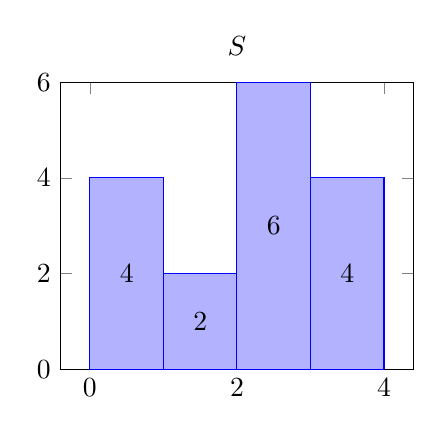
\begin{tikzpicture}
        \begin{axis}[
          width=0.5*\textwidth,
          title=$S$,
          ymin = 0,
          ymax=6,
          ]
          \addplot[
          ybar interval, 
          blue,fill=blue!30!white,
          ] plot coordinates
          {(0,4)(1,2)(2,6)(3,4)(4,4)};


    \node at (axis cs:0.5,2) {$4$};
    \node at (axis cs:1.5,1) {$2$};
    \node at (axis cs:2.5,3) {$6$};
    \node at (axis cs:3.5,2) {$4$};


     \end{axis}
      \end{tikzpicture}\qquad
     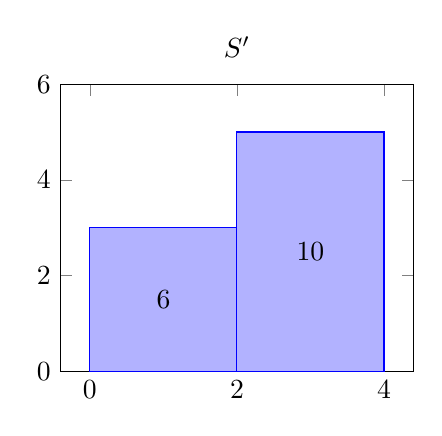
\begin{tikzpicture}
        \begin{axis}[
          width=0.5*\textwidth,
          title=$S'$,
          ymin = 0,
          ymax=6,
          ]

          \addplot[
          ybar interval, 
          blue,fill=blue!30!white,
          ] plot coordinates
          {(0,3)(2,5)(4,5)};

    \node at (axis cs:1,1.5) {$6$};
    \node at (axis cs:3,2.5) {$10$};


     \end{axis}
      \end{tikzpicture}


      \caption{Sèrie temporal amb àrea sota la corba i sèrie temporal
        resultant de la multiresolució amb agregació mitjana de la
        funció}
  \label{fig:multiresolucio:comptador}
\end{figure}






  \end{itemize}
  






  La multiresolució, però, no pot conservar la resolució del
  comptatge.  Com s'ha exposat a
  l'\autoref{ex:multireoslucio:informacio-subresolucions}, en
  consultes en què l'interval no es correspongui amb les resolucions
  emmagatzemades, els totals no seran els correctes que s'obtindrien
  de calcular amb les dades originals.  De fet, és el mateix problema
  que hem exposat que a partir d'un comptador no es poden deduir
  exactament energies que no s'han mesurat.


\end{example}

\todo{potser fer un exemple on es vegi com la multiresolució pot solucionar un problema d'inframostreig en els comptadors}




\begin{example}[Equivalències en l'agregació d'atributs]

  Hi ha casos en què és el mateix aplicar una funció d'agregació
  d'atributs que aplicar-ne una altra. Per exemple és el cas de la
  $\operatorname{mitjana}$\todo{falta definir a la taula} i el de la
  $\glssymbol{not:sgstm:meanzohe}$ per a sèries temporals regulars. 

  Sigui $S=\{m_0,\dotsc,m_k\}$, on $m_k=(t_k,v_k)$, una sèrie temporal
  regular de període $d$ i sigui $[t_a,t_b]$ un interval de temps on
  $t_a=T(\min(S))-d=t_0-d$ i $t_b=T(\max(S))=t_k$.  Demostrem que
  $\glssymbol{not:sgstm:meanzohe}(S,[t_a,t_b]) =
  \operatorname{mitjana}(S,[t_a,t_b])$.

  La mitjana aritmètica de la sèrie temporal és
  $\operatorname{mitjana}(S,[t_a,t_b])=\frac{v_0+\dotsb+v_k}{|S|}$
  
  La mitjana amb representació \gls{zohe} és
  $\glssymbol{not:sgstm:meanzohe}(S,[t_a,t_b])= \frac{1}{t_b-t_a} (
  v_0(t_0-t_a)+v_1(t_1-t_0)+\dotsb+ v_k(t_k-t_{k-1}) )$.

  Per ser regular, $t_1-t_0 = \dotsb = t_k-t_{k-1} = d$. A més
  $t_a=t_0-d$ i per tant $t_0-t_a = d$. També per ser regular,
  $t_k-t_0= t_k +(- t_{k-1} + t_{k-1}) + \dotsb + (- t_1 + t_1) - t_0
  = (|S|-1)d$ i per tant $t_b-t_a=t_k - (t_0 - d) = (|S|-1)d +d = |S|d$.

  Reescrivint, $\glssymbol{not:sgstm:meanzohe}(S,[t_a,t_b])=
  \frac{1}{|S|d} ( v_0d+v_1d+\dotsb+ v_kd ) = \frac{1}{|S|} (
  v_0+v_1+\dotsb+ v_k ) = \operatorname{mitjana}(S,[t_a,t_b])$.



  Així doncs, en una sèrie temporal regular es pot aplicar la
  $\operatorname{mitjana}$ com a equivalent a la
  $\glssymbol{not:sgstm:meanzohe}$; la
  \autoref{fig:multiresolucio:comptador} n'és un exemple. Un àmbit
  d'aplicació d'aquestes equivalències pot ser el de simplificar els
  càlculs en les consultes als \gls{SGSTM}, en els discs dels quals
  les subsèries temporals normalment s'emmagatzemen regulars.
  
\end{example}











% \section{Stream orientation}

% \todo{}
% * Dues variacions possibles interessants pels MTSMS:

 
%   - Buffers com a streams, sempre de mida fitada 
%   - Discos enllaçats





%%% Local Variables:
%%% TeX-master: "main"
%%% End:






%  LocalWords:  multiresolució multiresolucions
